\documentclass[a4paper]{article}

%% Language and font encodings
\usepackage[english]{babel}
\usepackage[utf8x]{inputenc}
\usepackage[T1]{fontenc}
\usepackage{graphicx}
\usepackage{float}       
%\usepackage{geometry}
\usepackage[left=4cm,right=3cm,top=3cm,bottom=2.5cm]{geometry}
\usepackage{vmargin}
\usepackage{fancyhdr}
\usepackage{epsfig}
\usepackage{eurosym}
\usepackage{url}
\graphicspath{ {figures/} }
\usepackage{array}
\usepackage{listings}
\usepackage{mathtools}

\newenvironment{Times}{\fontfamily{ptm}\selectfont}{}
\fancyhf{}
\pagestyle{fancy}
\fancyfoot[R]{\thepage}
\fancyhead[L]{\leftmark}
\usepackage{setspace}
\setstretch{1.5}

%Python code
\usepackage{listings}
\usepackage{color}

\definecolor{mygreen}{rgb}{0,0.6,0}
\definecolor{mygray}{rgb}{0.5,0.5,0.5}
\definecolor{mymauve}{rgb}{0.58,0,0.82}

\lstset{ %
  backgroundcolor=\color{white},   % choose the background color; you must add \usepackage{color} or \usepackage{xcolor}; should come as last argument
  basicstyle=\footnotesize,        % the size of the fonts that are used for the code
  breakatwhitespace=false,         % sets if automatic breaks should only happen at whitespace
  breaklines=true,                 % sets automatic line breaking
  captionpos=b,                    % sets the caption-position to bottom
  commentstyle=\color{mygreen},    % comment style
  deletekeywords={...},            % if you want to delete keywords from the given language
  escapeinside={\%*}{*)},          % if you want to add LaTeX within your code
  extendedchars=true,              % lets you use non-ASCII characters; for 8-bits encodings only, does not work with UTF-8
  frame=single,                    % adds a frame around the code
  keepspaces=true,                 % keeps spaces in text, useful for keeping indentation of code (possibly needs columns=flexible)
  keywordstyle=\color{blue},       % keyword style
  language=Python,                 % the language of the code
  morekeywords={*,...},            % if you want to add more keywords to the set
  numbers=left,                    % where to put the line-numbers; possible values are (none, left, right)
  numbersep=5pt,                   % how far the line-numbers are from the code
  numberstyle=\tiny\color{mygray}, % the style that is used for the line-numbers
  rulecolor=\color{black},         % if not set, the frame-color may be changed on line-breaks within not-black text (e.g. comments (green here))
  showspaces=false,                % show spaces everywhere adding particular underscores; it overrides 'showstringspaces'
  showstringspaces=false,          % underline spaces within strings only
  showtabs=false,                  % show tabs within strings adding particular underscores
  stepnumber=1,                    % the step between two line-numbers. If it's 1, each line will be numbered
  stringstyle=\color{mymauve},     % string literal style
  tabsize=2,                       % sets default tabsize to 2 spaces
  title=\lstname                   % show the filename of files included with \lstinputlisting; also try caption instead of title
}

\lstdefinestyle{customc}{
  belowcaptionskip=1\baselineskip,
  breaklines=true,
  frame=L,
  xleftmargin=\parindent,
  language=C,
  showstringspaces=false,
  basicstyle=\footnotesize\ttfamily,
  keywordstyle=\bfseries\color{green!40!black},
  commentstyle=\itshape\color{purple!40!black},
  identifierstyle=\color{blue},
  stringstyle=\color{orange},
}

\lstdefinestyle{customasm}{
  belowcaptionskip=1\baselineskip,
  frame=L,
  xleftmargin=\parindent,
  language=[x86masm]Assembler,
  basicstyle=\footnotesize\ttfamily,
  commentstyle=\itshape\color{purple!40!black},
}

\title{\underline{\textbf{\begin{Huge}Network\end{Huge}}}\\\vspace{1cm}
    \begin{huge}
        \textbf{Client / Server communication study}
    \end{huge}\\}
    
\author{
        Tom Moulard (16920041)
        \date{}
        }
        
        
\begin{document}
\maketitle
\begin{center}
\vspace{1cm}
\date{2017 March 4}
\vspace{2cm}\\
\end{center}    
    \thispagestyle{empty}

\newpage{}

\tableofcontents
\thispagestyle{empty}


\newpage
\section{Introduction}

When studying how computers talk to each other. The best way to understand it is to see what they actually say to each others.
For this, I created a small Python Program to make two computer communicate, one as a server and the other as a client sending a file to the server.
\par We are going to see who this program works in details and how the two computers have managed to talk to each other in order to send this file.  

\newpage
\section{Code}

\subsection{Actual code}
\lstinputlisting[language=Python]{customIperf.py}

\subsection{Explanations}
%This section should explain how the code works
This code is really simple to understand, it initiate the connection between two computers and allow one to send a file to the other.
\par Indeed, to make this works, we need to have two computers able to interpret python code.
And we need to establish which one is going to be the server and with one the client.
Once it is done, we have to run the interpreter in a terminal like this : \textit{python3 customIperf.py -s} for the server.\\
For the client you should have a little more knowledge : you need to know the IP address of the server. Internal or external, it is up to you to choose depending on how these two computers can talk with each other. And then you can run this : \textit{python3 customIperf.py -c <Server IP address> <file>}. The file can be every file on you computer, it will e stored on the server with the same name.

\par The code is really easy to follow, when running the code, the first thing is to determine what this computer is going to be : \textit{-s} for server, \textit{-c} for client.


\subsubsection*{Server}

\par Once the computer knows that it is going to be the server it will open the pre-defined port to allow clients to connect to him and will wait for a client signal to establish the connection.\\
When a client tries to connect to the server the server will gather informations about the client to be able to communicate with him.\\
Once it is done, the server will wait to receive a number which correspond of the length of the fileName. then it will listen the fileName using it's length and will create a new file with this fileName.\\
After the document has been created, the server will gather all informations going through the network buffer to watch rights packets to add to the file. and when the server sees a EOF signal, it closes the document and closes the connection with the client.
Now another client can connect to the server to send him another file.

\begin{figure}
\centering
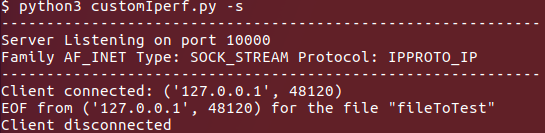
\includegraphics[width=0.6\textwidth]{serverSide.png}
\caption{Server side output}
\end{figure}

\subsubsection*{client}

\par The client is pretty much the opposite of the server.\\
The client is going to try to establish the connection with the ip/port given by the user to the server. If there is nothing, the client will just wait for the server to be started.\\
when the connection is established, it will send the length of the fileName, the fileName and then the document.

\begin{figure}
\centering
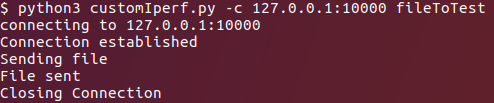
\includegraphics[width=0.6\textwidth]{clientSide.png}
\caption{Client side output}
\end{figure}

\newpage
\section{Interpretation}
%This looks at wireshark screens and explain what the f*** appended

\par Now that the easy stuff is gone, we can look more in depth on what is really important here: network.

\begin{figure}
\centering
\includegraphics[width=1\textwidth]{WS_-_General_lookup.png}
\caption{Wireshark output}
\end{figure}

This is showing to main display of Wireshark for this file sharing.
We can see the different ports.
Since i am running both the client and the server from my computer they all have the same ip, just the port changes : 10000 for the server and 56158 for the client.\\
Just by looking at it without any detail we can see three distinct part: The Authentication Part (or the Connection Establishment Part), The Data Transfer Part and The Close connection Part.

\subsection{The Authentication Part}

\subsubsection{The (famous) Three Way Handshake}

\subsection{The Data Transfer Part}

\subsection{The Close Connection Part}

\newpage 
\section{Conclusion}

\newpage

\listoffigures

\end{document}